\chapter{Implementation}\label{ch:implementation}

% --------------------
% --- TECHNOLOGIES ---
% --------------------
\section{Technologies}\label{sec:technologies}
A number of technologies assisted in the developing process of the application. In this section, each of these technologies is discussed to explain its importance.

\subsection{ReactJS}\label{sec:reactjs}
ReactJS is an open source library to create user interfaces\footnote{\url{https://reactjs.org/index.html}}. One of its main goals is to provide the best possible rendering performances\footnote{\url{https://medium.com/@thinkwik/why-reactjs-is-gaining-so-much-popularity-these-days-c3aa686ec0b3}}. Performance is high because ReactJS allows developers to break down the user interface into different components. Each component has its own \textit{state}, which contains information about the content of the component. This state can be updated while the application is running and if such an update is made, only this component is re-rendered instead of re-rendering the complete UI\footnote{\url{https://facebook.github.io/react/docs/why-react.html}}. Hence, this involves a huge benefit for the performance. Next to that, it is also not very hard to learn to code in React when comparing to other frameworks (e.g. AngularJS). If the developer knows HTML and JavaScript, he will be able to code in ReactJS quickly.\\

Because of these benefits, ReactJS is the framework in which the GuideaMaps application is implemented. Each node is considered as a separate and unique React Component. The most important reason for implementing the nodes like this is performance: if the state of the node is updated, only this node is re-rendered and not the complete UI.

\subsection{d3}\label{sec:d3}
Another helpful tool is d3. With d3-hierarchy\footnote{\url{https://github.com/d3/d3-hierarchy}}, it is possible to transform JSON-data into hierarchical data. Having this kind of data makes it much easier to create a tree- or cluster-structure. In the case of GuideaMaps, a clustered visualization is very useful. The \textit{main}-node (a.k.a. the root node) is then positioned at the center, such that its child nodes can be places around it. Hence, the farther a node is away from the center, the lower it is in the hierarchy. Also, the visualization will not be messed up by positioning the nodes in this way, because every node has exactly one parent. This means there won't be a spaghetti of links where you cannot see which node the link comes from and which node it is pointing to.

\subsection{Tailwind CSS}\label{sec:tailwind}
The style of the application is very important for the end user. Everything should look pretty and, as already mentioned in section \ref{sec:usability-requirements}, the possibilities should be straightforward and visible. While developing and creating a beautiful style for applications and websites, the code for these styles can become a big part of the implementation. Hence, a good framework is necessary to reduce the lines of code to a reasonable number. It also helps to improve the readability of the code.\\

Tailwind CSS\footnote{\url{https://tailwindcss.com/}} is a framework that assists developers to style their application. The difference with more famous frameworks, like Bootstrap, is that Tailwind CSS has no default theme. If you want to use a Bootstrap-feature, this eventually comes along with other features you don't always wanted and it can be quite hard to undo the part you didn't ask for. With tailwind on the other hand, you can grab only the features you want, without side-effects. Figure \ref{fig:examplecode-tailwindcss} shows an example with two small listings. The first uses inline style while the second makes use of tailwindCSS.\\

\begin{figure}[H]
	\begin{minipage}[b]{0.5\textwidth}
 		\centering
  		\begin{minted}[linenos, escapeinside=||]{html}
<div
  style={{
    position: absolute|,|
    border: 1px solid black|,|
    borderRadius: O.25rem|,|
    padding: 0.5rem|,|
  }}
/>
		\end{minted}
		\label{lst:no-tailwind}
		\captionof{lstlisting}{Normal CSS, no tailwind.}
	\end{minipage}
 	\begin{minipage}[b]{0.5\textwidth}
  		\centering
		\begin{minted}[breaklines, escapeinside=||]{html}
<div
    className={
      |'|absolute border border-solid border-black rounded p-2|'|
    }
/>
		\end{minted}
		\label{lst:tailwind}
 	 	\captionof{lstlisting}{With tailwind CSS.}
 	\end{minipage}
	\caption{Difference when using tailwind CSS or not.}
	\label{fig:examplecode-tailwindcss}
\end{figure}

The figure illustrates the difference to implement four css property-value pairs in normal css and implementing the same four with tailwind. In the case of normal css, we need four lines of code to retrieve the intended result. On the other hand, with tailwind css, we add some classes providing the same style. The classnames can be placed on a single line instead of four. This example proves that the number of lines can be decreased.





% ---------------------
% ----- STRUCTURE -----
% ---------------------
\section{Structure}\label{sec:structure}
With the technologies mentioned in the previous section, the most important pillars the application relies on are discussed. Now it is time to have a look at the structure of the code, such that it is clear how all elements work together. Figure \ref{fig:overall-structure} shows a visualization of the structure of the code.
\begin{figure}[H]
	\centering
	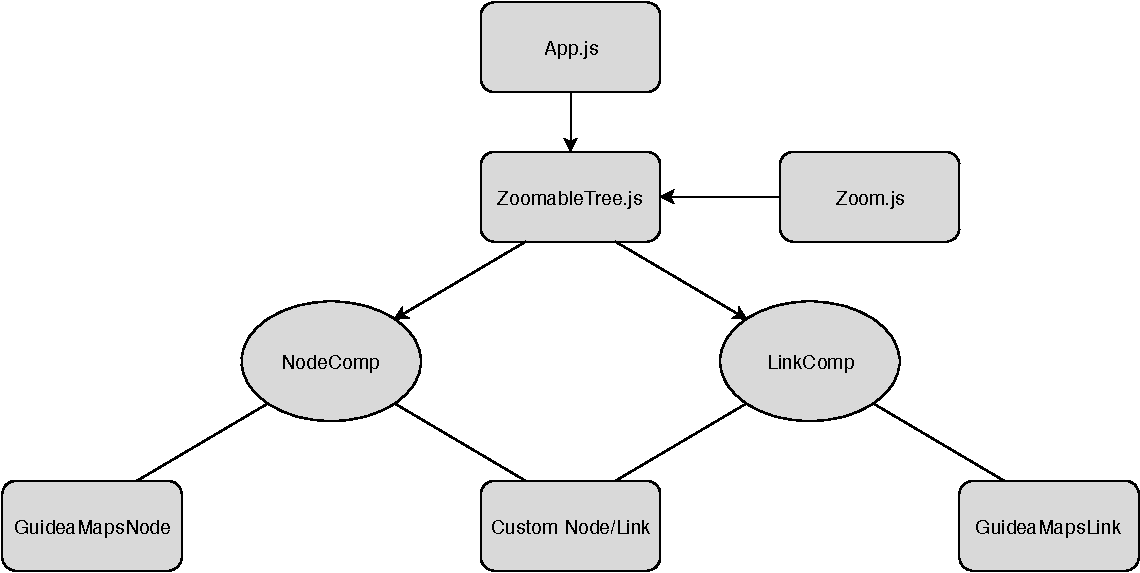
\includegraphics[width=\linewidth]{thesis-architecture.pdf}
	\caption{Structure of the application.}
	\label{fig:overall-structure}
\end{figure}

The application is developed in such a way that it can be used as a library for other purposes than GuideaMaps as well. The general, always-returning part of the code can be found in App.js, ZoomableTree.js and Zoom.js, where the layout of the nodes is defined as well as the implementation to allow the user to zoom the visualization in and out. When talking about the library, the layer of the NodeComp and LinkComp is very interesting and important. For the GuideaMaps, an implementation for a GMNode and GMLink is provided. Each implementation describes what every node and every link should look like in the visualization \textcolor{red}{(TODO: provide more explanation about this somewhere else + coupling with requirements and RQs)}.\\

The strength of the library can be seen when a particular user would like to have a different representation for the nodes or the links or both. In that case, new components (e.g. MyCustomNode and MyCustomLink) should be implemented. In the code, only one line should be adapted: in App.js, ZoomableTree is called with a certain number of props. Two of these props are NodeComp and LinkComp, which are set to GMNode and GMLink, respectively, by default. Hence, the only action that is required to \textit{plug in} an other component is replacing GMNode by MyCustomNode and GMLink by MyCustomLink. Figure \ref{fig:examplecode-library} shows the part of the code in App.js that should be adapted as explained. Note that NodeComp and LinkComp are not the only props that are passed to ZoomableTree. The others are omitted to improve the readability.

\begin{figure}[H]
	\begin{minipage}{0.5\textwidth}
 		 \centering
		 \begin{minted}[linenos]{html}
<ZoomableTree
    NodeComp={GMNode}
    LinkComp={GMLink}
/>
		\end{minted}
		\label{lst:default-components}
		\captionof{lstlisting}{Default components.}
	\end{minipage}
 	\begin{minipage}{0.5\textwidth}
  		\centering
  		\begin{minted}{html}
<ZoomableTree
    NodeComp={MyCustomNode}
    LinkComp={MyCustomLink}
/>
		\end{minted}
		\label{lst:custom-components}
 	 	\captionof{lstlisting}{Custom components.}
 	\end{minipage}
	\caption{Two listings showing how to use the library.}
	\label{fig:examplecode-library}
 	%\captionof{figure}{Two listings showing the difference between the default and custom use of the library.}
\end{figure}





% ------------------------------
% ----- GUIDEAMAPS DETAILS -----
% ------------------------------
\section{GuideaMaps}
Now the overview of the structure of the application is discussed, we will consider the implementation details of the GuideaMaps visualisation in this section.
\begin{figure}[H]
	\centering
	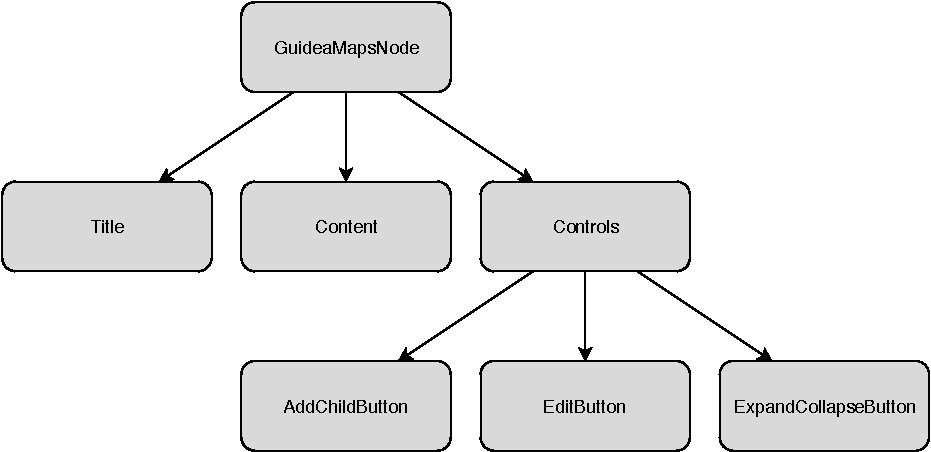
\includegraphics[width=\linewidth]{GMStructure.pdf}
	\caption{Structure of GuideaMapsNode.}
	\label{fig:gmnodestructure}
\end{figure}

As you can see in figure \ref{fig:gmnodestructure}, the structure of a GuideaMapsNode node quite easy.




% ------------------------------
% ----- GUIDEAMAPS DETAILS -----
% ------------------------------
\section{Other visualizations}














